\documentclass{beamer}

\title{Searching for Hidden Objects}
\subtitle{Looking for custard cups in mixing bowls, and not the other way around}
\author{Troy Astorino, Neil Forrester}
\date{April 10, 2013}
\institute[6.834 -- MIT]{Cognitive Robotics \\ Massachusetts Institute of Technology}

\usepackage{graphicx}
\usepackage{amsmath}

\usetheme{CambridgeUS}
\usecolortheme{beaver}
\setbeamertemplate{section in toc}[square]
%\setbeamercolor{section number projected}[bg=black, fg=red]
\setbeamertemplate{navigation symbols}{} % remove navigation symbols

% \argmax operator
\DeclareMathOperator*{\argmax}{arg\,max}

% \norm{n}{stuff} is the L-n norm of stuff
\providecommand{\norm}[2]{\lVert#2\rVert_#1}

\newcommand{\overlay}[3]{\includegraphics<#3>[scale=#2]{img/#1.png}}
\newcommand{\overlayL}[2]{\overlay{#1}{0.5}{#2}}
\newcommand{\overlayM}[2]{\overlay{#1}{0.3}{#2}}

% macros for including shape pictures at various scales (Large, Medium, Small)
\def \spL [#1]{\overlayL{#1}{1}}
\def \spM [#1]{\overlayM{#1}{1}}
\def \spS [#1]{\overlay{#1}{0.15}{1}}

% uncomment this with your current latex file to only compile it
%\includeonly{mcmc}
\begin{document}

\section{Introduction}
\begin{frame}
  \maketitle
\end{frame}

\begin{frame}
  \frametitle{The necessity of manipulation-based search}
  \begin{center}
    \includegraphics[width=3.2in]{img/robot_in_kitchen.jpg}

    \tiny{Original image courtesy of Wendy Rogers/Georgia Tech.}
  \end{center}
\end{frame}

\begin{frame}
  \frametitle{Lecture Goals}
  We would like you to\ldots
  \begin{itemize}
    \item Gain insight on how problems can be modeled in probabalistic robotics.
    \item Learn probability distributions commonly applied in robotics.
    \item Learn the basics of Markov chain Monte Carlo sampling algorithms and
      why they are used.
    \item Gain a deeper understanding of how to use Bayesian inference for
      cognitive robotic applications.
    \item Learn how these techniques are applied on an interesting problem domain:
      manipulation based search.
  \end{itemize}
\end{frame}

\begin{frame}
  \frametitle{Outline}
  \tableofcontents
\end{frame}

\begin{frame}
  \frametitle{The necessity of manipulation-based search}
  \begin{center}
    \includegraphics[height=2.7in]{img/kitchen-organization-fake.jpg}

    \tiny{Original image courtesy of personalorganizing.about.com.}
  \end{center}
\end{frame}

\begin{frame}
  \frametitle{The necessity of manipulation-based search}
  \vspace{-0.3in}
  \begin{columns}
    \begin{column}{0.6\textwidth}
      \begin{itemize}
        \item Some things are hidden behind other things.
        \item We have to remove items in front to see items in back.
        \item The cookie tray and the rat poison are not likely to be on the
          same shelf.
        \item Blenders will not fit on all shelves.
      \end{itemize}
    \end{column}
    \begin{column}{0.4\textwidth}
      \begin{center}
        \includegraphics[height=2.7in]{img/kitchen-organization.jpg}

        \tiny{Original image courtesy of shilloh.com.}
      \end{center}
    \end{column}
  \end{columns}
\end{frame}


\AtBeginSection[]
{
 \frametitle{Outline}
 \tableofcontents[currentsection]
}
\section{Techniques for Probabilistic Reasoning}
\subsection{Probability Distributions in Robotics}
\include{probability-distributions}

\subsection{Maximum Likelihood Estimation}
\include{ml}

\subsection{Markov chain Monte Carlo}
\include{mcmc}

\section{Manipulation-based Search for Occluded Objects}
\begin{frame}
  \frametitle{Remembering the problem}
  \begin{center}
    \includegraphics[width=3.2in]{img/robot_in_kitchen.jpg}

    \tiny{Original image courtesy of Wendy Rogers/Georgia Tech.}
  \end{center}
\end{frame}

\begin{frame}
  \frametitle{State of research}
  \begin{itemize}
  \item With the advent of sampling-based planning methods, robotic
    manipulation of arbitrary objects has become feasible.
  \item The solving of SLAM means that moving through and mapping out
    environments is no longer a barrier to robotic applications.
  \item Active visual search for objects out in the open is nearly a solved
    problem.
  \item Current research on objects occurrence models shows that certain types of
    objects appear together more often than others, and certain types of objects
    are unlikely to appear together.
  \end{itemize}
\end{frame}

\begin{frame}
  \frametitle{Assumptions for the following treatment}
  \begin{itemize}
  \item There are no errors in the visual identification and classification of objects.
  \item The robot can successfully complete any movement and manipulation task,
    but motions take time, and are therefore expensive.
  \item The set of object types in the world is finite.
  \end{itemize}
\end{frame}

\begin{frame}
  \frametitle{Formulation of the problem}
  \begin{center}
    \vspace{-0.13in}
    Set of containers: $\{c_l\}$

    \spL[3-unknown-containers]

    Set of object types: $\{t_i\}$

    \spL[shape-universe-small]

    We want to find an object of type $q$ (the query type).

    \spL[blue-circle]

  \end{center}
\end{frame}

\begin{frame}
  \frametitle{Where is \spM[blue-circle]?}
  \begin{center}
    \spL[3-partially-observed-containers]

    \vspace{0.3in}

    Given that we have observed objects of types $\{t_{o_j}\}$ \\
    in container $c$, what is $\mathrm{P}(q \in c \, | \, \{t_{o_j}\})$ ?
  \end{center}
\end{frame}



\subsection{Generative Model of Container Contents}
\subsubsection*{Co-occurrences}
\include{composition}

\include{prior}

\include{posterior}

\subsubsection*{Spatial constraints}
\include{packing}

\subsection{Search planning}
\include{search}

\subsection{Results}
\begin{frame}
  \frametitle{Comparison of search strategies}
  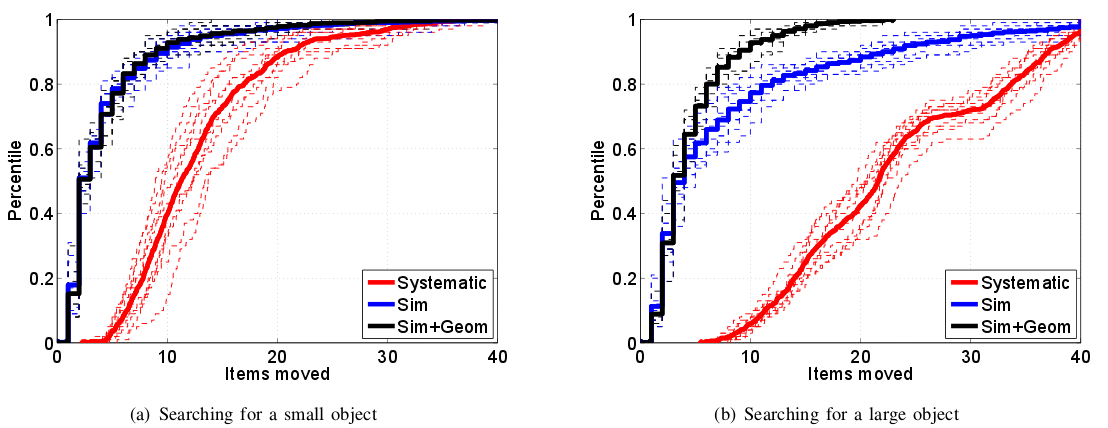
\includegraphics[width=\textwidth]{img/search-strategies.png}
\end{frame}


\subsection{Applications}
\begin{frame}
  \frametitle{Applications of the algorithm presented}
  \begin{columns}
    \begin{column}{0.5\textwidth}
    \includegraphics[width=\textwidth]{img/laboratory.jpg}

    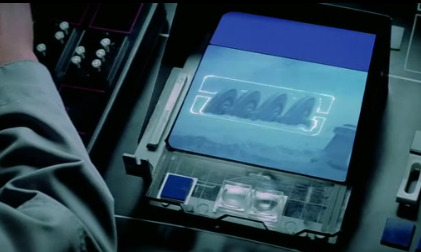
\includegraphics[width=\textwidth]{img/hoth.png}
    \end{column}
    \begin{column}{0.5\textwidth}
    \includegraphics[width=\textwidth]{img/boxes.jpg}

    \includegraphics[width=\textwidth]{img/tanks.jpg}
    \end{column}
  \end{columns}
\end{frame}


\section{Conclusion}
\begin{frame}
  \frametitle{Techniques (we hope) you've learned}
  Hopefully you have \ldots
  \begin{itemize}
    \item Learned how to make robots find the salt when you ask for it.
    \item Seen how problems like search can be performed in an
          intelligent way through Bayesian reasoning,
          taking constraints like limited space into account.
    \item Gained a basic familliarity with some useful techniques for working with probability distributions.
  \end{itemize}
\end{frame}

\begin{frame}
\nocite{*}
\bibliographystyle{ieeetr}
\bibliography{sources}
\end{frame}


\end{document}